Guidelines:
Seiten: 50
Präsentation: 30 min / Disskusion: 15 min
sonarqube als code scan

\section{Einleitung}

\subsection{Motivation}
\subsection{Unternehmen}
\subsection{Zielsetzung}
vielleicht im kapitel motivation?
\subsection{Aufbau der Arbeit}

- Outline your work such that readers who have not read subsequent chapters get an idea of what
  - your "problem domain" is (e.g. the software quality department of some company or the overarching research project you are working in)
  - the situation is (e.g. software tests at some company are done in complete manual fash-ion)
  - the complication / problem is (e.g. hotfixes have to be deployed totally untested in pro-duction)
  - what your approach is (e.g. establishing a concept and tool evaluation for continuously improving code coverage of automated tests)
  - what beyond the scope of your thesis is (e.g. also implementing a CICD pipeline)
  - what the actual core results are (e.g. how many tools have been evaluated)

From that it must clear, what your thesis'contribution actually is. Please delineate your contribution from every concept, method, tool, framework or whatever implementation your thesis took for granted and is built upon.

This chapter deliberately anticipates contents of the latter chapters but please refrain from spe-cific technical termsof your application domain or solution here. Trade technical accuracy for com-mon comprehensibility here. Write this chapter as a "management summary" and do not spend more than two to three pages here.

Also explain structure of your thesis, i.e., summarize the contents of each chapter in one sentence or paragraph and describe the overarching storyline, i.e., how chapters build upon each other.

\section{Anwendungsfeld Internet of Things}

ein grobes beispiel einet mqtt broker -> client anwendungs beschreiben
ein / mehrere broker (mehrere millionen clients zb MAN, darf ich das erzählen ?)
sehr viele iot clients
big downstream clients -> backends
industrial bereich

- Describe the (business) domain of your work. Ask yourself: What does the common reader need to know about the domain in order to understand the results of your work? For example, if you work contributes to the claim handling process of some insurance company, describe the common claim handling process.
- Please refrain from meandering explanations about details that have no relevance for later chapters (just in order to increase your page count).
- The header "Domain / Anwendungsfeld" is supposed to be replaced or extended with some more specific header like: "Domain 'Claim handling'"

\section{Technische Grundlagen} - Technologische Grundlagen - Grundlagen /

\subsection{MQTT}
%https://www.paessler.com/it-explained/mqtt
%https://www.hivemq.com/blog/how-to-get-started-with-mqtt/
\acrfull{mqtt} wurde ursprünglich von Doktor Andy Stanford-Clark und Arlen Nipper im Jahr 1999 entworfen um Gas- und Ölpiplines zu überwachen. Diese lagen oftmals an entlegenen Orten wie zum Beispiel auf Übersee und konnten nicht mit Radiowellen oder einem Kabel zum Festland erreicht werden. Zu dieser Zeit war die einzige Option eine Satellitenkommunikation, welche auf Datendurchsatz abgerechnet wurde, damit die Sensoren ihre Daten an einen Server schicken können. Bei mehreren tausend Sensoren wurde somit ein Protokoll benötigt, welches die Daten zuverlässig mit minimaler Bandbreite an die Server auf dem Festland übermitteln kann.
MQTT wurde im Jahr 2013 von der OASIS (Organization for the Advancement of Structured Information Standards) als Open Source standatisiert.

\Gls{latex} test here.

MQTT ist ein Layer 7 'Publish and Subscribe' Protkoll, welches auf TCP / IP aufsetzt. Anders als das Request / Response Paradigma bei HTTP ist MQTT Event gesteuert und erlaubt Nachrichten direkt an einen bestimmten Client zu schicken. Dadurch muss dieser nicht periodisch nach neuen Nachrichten fragen und minimiert somit den Datendurchsatz.
In dieser Architektur gibt es zwei unterschiedliche Systeme: Clients und Broker. Clients können Nachrichten veröffentlichen, konsumieren oder beides gleichzeitig.
Ein Broker empfängt alle eingehenden Nachrichten von den Clients und leitet diese gegebenenfalls an andere Clients weiter. Clients können niemals direkt untereinander kommunizieren und müssen immer einen Broker ansprechen.

Es gibt derzeit zwei Versionen der MQTT Spezifikation: \verb|3.1.1| und \verb|5|. Alle Referenzen, wenn nicht anders bezeichnet, beziehen sich auf die aktuelle Version \verb|5| des Protokolls.

Um den Datendurchsatz zu verringern hat MQTT einen fixen Header von 2 Byte. Die Paketgrö{\ss}e eines Sensorwertes, welcher aus einem in C geschriebenen 32-Bit Integer Wert besteht, beträgt somit nur 6 Byte.
% TODO stimmt nicht! das topic muss auch noch dazu denke ich
% TODO vielleicht ein http vergleich?
% https://stackoverflow.com/questions/9233316/what-is-the-smallest-possible-http-and-https-data-request
% TODO bild von sensoren / broker / downstream clients

Eine MQTT Nachricht kann drei verschiedene QoS (Quality of Service) level haben. Mit diesen kann ein Client bestimmen wie zuverslässig seine Nachricht zugestellt wird.
\begin{itemize}
    \item QoS 1: Maximal eine Zustellung der Nachricht.
    \item QoS 2: Mindestens eine Zustellung der Nachricht. Der Subscriber muss eine Bestätigung an der Broker schicken sobald er die Nachricht erhalten hat.
    \item QoS 3: Genau eine Zustellung der Nachricht. Erfordert einen Vier-Schritte Handshake zwischen Broker und Subscriber.
\end{itemize}

Nachrichten werden auf einem Broker immer in hieraschich aufgebauten Themen publiziert. Diese werden mit einem Schrägstrich (\verb|/|) getrennt und sehen zum Beispiel wie folgt aus: \verb|sensors/temperature|. Clients müssen beim publizieren oder subskribieren immer ein Thema angeben. Anhand dieses Themas kann der Broker entscheiden an welche Clients der Broker ein Paket weiterleiten soll. Beim subskribieren kann entweder ein spezifisches Thema oder eine kombination aus Thema und Wildcard verwendet werden. Bei einer Wildcard werden zwischen den folgenden unterschieden:
% TODO cite mqtt specification that there must be a topic
\begin{itemize}
    \item Multi-level '\verb|#|': Wenn ein Client auf \verb|sensors/#| subskribiert, erhält er Nachrichten von folgenden Themen:
    \begin{itemize}
        \item \verb|sensors|
        \item \verb|sensors/temperature|
        \item \verb|sensors/temperature/celcius|
        \item \verb|sensors/waterlevel|
    \end{itemize}
    \item Single-level '\verb|+|': Wenn ein Client auf \verb|sensors/+| subskribiert, erhält er hingegen nur Nachrichten von folgenden Themen:
    \begin{itemize}
        \item \verb|sensors/temperature|
        \item \verb|sensors/waterlevel|
    \end{itemize}
\end{itemize}



\newpage




%standard v5: https://docs.oasis-open.org/mqtt/mqtt/v5.0/mqtt-v5.0.html
MQTT is a Client Server publish/subscribe messaging transport protocol. It is light weight, open, simple, and designed to be easy to implement. These characteristics make it ideal for use in many situations, including constrained environments such as for communication in Machine to Machine (M2M) and Internet of Things (IoT) contexts where a small code footprint is required and/or network bandwidth is at a premium.

The protocol runs over TCP/IP, or over other network protocols that provide ordered, lossless, bi-directional connections. Its features include:

·         Use of the publish/subscribe message pattern which provides one-to-many message distribution and decoupling of applications.

·         A messaging transport that is agnostic to the content of the payload.

·         Three qualities of service for message delivery:

o    "At most once", where messages are delivered according to the best efforts of the operating environment. Message loss can occur. This level could be used, for example, with ambient sensor data where it does not matter if an individual reading is lost as the next one will be published soon after.

o    "At least once", where messages are assured to arrive but duplicates can occur.

o    "Exactly once", where messages are assured to arrive exactly once. This level could be used, for example, with billing systems where duplicate or lost messages could lead to incorrect charges being applied.

·         A small transport overhead and protocol exchanges minimized to reduce network traffic.

·         A mechanism to notify interested parties when an abnormal disconnection occurs.

\subsubsection{Shared Subscriptions}
\subsection{HiveMQ Broker}
\subsubsection{HiveMQ Cluster}
\subsection{Load Balancing}
was für load balancer gibt es ?
\subsection{Envoy}
vielleicht hier noch kein envoy ? ist dies grundlage oder teil der arbeit das wir uns für envoy entscheiden ?

If your work makes use of existing non-standard systems, tools, frameworks, librariesetc. describe these as well. However, just give a broad overview and delve just into those details that are crucial for the understanding of the following chapters. For standard sys-tems, tools, frameworks, and libraries please refer to its authoritative documentation. Youare not supposed to give an thorough introduction into, e.g., Java or ReactJS.

\section{Problembeschreibung}

\subsection{Cluster Discovery}
discovery that works with hivemq cluster discovery (dns)
es kommen immer wieder neue nodes hinzu / weg zb bei rolling updates
load balancer muss diese nodes dynamisch hinzufüger oder entfernen
hivemq ist in der lage dynamische cluster joins zu machen also muss der lb auch in der lage dazu sein

\subsection{Langlebige TCP Verbindungen}
ein LB darf die tcp connections nicht terminieren bei einem update oder config änderung
mqtt setzt auf langlebiege tcp verbindungen! nicht wie bei http! bei http -> drain
-> ein drain bei mqtt kann tage dauern

load balancer with data plane api -> good docs
\subsection{Persistent Client Session}
mqtt clients haben viel session auf dem broker
bei einem reconnect wird ein client takeover ausgeführt -> teuer
clients möglichst immer zum selben broker routen
problem: iot clients haben oft sich ändernde ip adressen zb mobile geräte wie autos
\subsubsection{Client Takeover}
sehr teuer! die persistent client informationen müssen umgezogen werden auf neuen broker

\subsection{Ungleiche Lastverteilung}
mqtt clients sind unterschiedlich teuer (nicht wie bei http)
beispiel: wildcard subscription

\subsubsection{Downstream Clients}
\subsubsection{Lightweight Clients}
\subsubsection{Wildcard Subscriptions}

- Describe insufficiencies your project or thesis aims at. Example: "The automated parts of the claim handling process are susceptible to changes. Each change requires lots of man-ual steps in order to deploy these changes into production."
- Do not take the term "problem" too literal. Sometimes, your project or thesis just aims at im-proving a good status quo or pursues new waysand opportunities that arise due to new technological advances or trends. In this case, describe the status quo and where the op-portunities for improvement are.
- Exemplify things! Describe the problem / status quo by means of a specific scenario with concrete steps, concrete input and output data, etc., supported by expressive figures. Do not be afraid that the reader might think that your solution just works for that particular sce-nario. In general, readers can abstract from concrete details much easier that to envisionconcrete scenarios by interpreting overly generic, vague, meandering text passages. (More-over, writing in vague terms also leaves the impression that the writer either did not under-stand the problem for him- or herself or tries to blow up mundane issues.)

\section{Vobereiten und verwandte Arbeiten}
vielleicht brauche ich diese sektion gar nicht ?

\subsection{Load Balancer}
was für load balancer gibt es? was haben diese für eigenschaften?

\subsection{Shared Subscriptions}
diese lösen das problem der teuren clients ABER clients müssen dann möglichst optimal auf die broker verteilt werden
-> load balancer

iot mqtt threat model ? maybe show this ?

- If your work is based on preliminary work, then outline this preliminary work: "The de-ployment into production is itself semi-automatic. In a continuous integration pipeline..."
- Do some research forrelated work, e.g., commercial products, research prototypes or con-ceptual research that have the same or similar objectives like your work. Compare and de-lineate your work with/from the related work.
- Keep an eye on the proper citation of the works you are describing
- Conclude this chapter with some insufficiencies or shortcomings of the preliminary or related work. This should motivate the necessity of your work.

\section{Lösungskonzept}
nur das konzept WIE ich das lösen will zb. man kann wie clientid parsen mit einem WASM modul
in der nächsten section zeige ich dann den eigentlichen code welcher dies tut

\subsection{Envoy}
\subsubsection{Data-Plane API}
\subsubsection{Hot Restart}

\subsection{DNS Service Discovery}

\subsection{Weighted Round Robin}
\subsubsection{Overload Protection}
\subsubsection{Client Credits}
\subsubsection{Global Tasks}

\subsection{Sticky Session with Client ID}
\subsubsection{MQTT CONNECT}
\subsubsection{Envoy WASM Network Filter}

- This is supposed to be the core of your thesis or project. Describe your work from a con-ceptual viewpoint.
- Example: In case you have developed some prototypical tool in your bachelor thesis, demonstrate how it is employed in its business context. More concrete example: Assume that your contribution is a Maven-Build-Plugin that further automates the deployment of changes to the claim handling process into production. In this case show how the plugin is integrated in the overall (continuous) integration and deployment process, which human ac-tors are involved, which external systems and so on. Elaborate on subtle edge cases you had to deal with, e.g., possible outages of external systems.
- Usedi  agramswhere appropriate. Standard notations are better than informal box-and-line-diagrams. Typical standard notations for a solution concept are
  - Business Process Modelling Notation (BPMN) or UML activity diagrams, that depict a workflow in which your tool is used
  - UML component diagrams, where your tool is represented by just a single component (without its ingredients) together with connected external systems

\section{Architektur und Implementation}

\subsection{Envoy}
\subsubsection{Golang Data-Plane}
\subsubsection{DNS Service Discovery}
\subsubsection{HiveMQ Metriken}
\subsubsection{Weighted Round Robin}
\subsubsection{ClientID Network Filter}

\subsection{Deployment}
\subsubsection{HiveMQ}
\subsubsection{Envoy}

- Describe the realization of your concepts, in case you have actually developed some-thing.
- Elaborate on the software architecture of your tool, in case you have developed one. Use nested UML packages, components, and interfaces in a component diagram.
- If applicable, show the deploymentof your tool in a production environment. Use UML's deployment diagram notation.
- It must be clear from the architecture, what your thesis contributes and what it takes for granted like existing systems, code bases, libraries and frameworks. For example, you can decorate the components in a UML component diagram that you have implemented and those that you just used.
- Do not delve into ordinary details by, e.g., intensively describing a "p lain old Java-object (POJO)" in all its dreary getter-setter-details. Instead pick some interesting details and de-scribe them, e.g.,
  - if   you made extensive use of a certain design pattern, describe a single concrete appli-cation of it using, e.g., UML class diagrams or
  - if your work involves a complicated conversation pattern or protocol, explained it using a UML sequence diagram, state chart, activity diagram and the like or
  - if you have developed a central and canny algorithm, you may even show its implemen-tation in, e.g., Java code.
- Show how the result of your work actually looks like. In case of a tool, provide some screenshots together with some explanatory text.
- Describe the quantity of your work, e.g., in terms of lines of code or classes etc. Please just count your own hand-crafted code but not previously existing, imported or generated code.
- Describe the quality of your work, e.g., if you have developed a large web application, run some performance tests, depicts results and draw conclusions from them.

\section{Erprobung}

\subsection{Lastverteilung}

If possible, do an (external) evaluation of your work. If you have developed some kind of tool, let us-ers test it, gather their feedback and describe that here. (Negative feedback will not contribute to a downgrading).

\section{Zeitplanung und Arbeitspakete}

- In the initiation phase, we agree on work packages. Give a (tabular overview) of which work packages have been finalized
  - to what degree
  - and in which time frame
- Please described the unforeseen difficulties that resulted in unfinished or abandoned work packages


\section{Ausblick}

- Again, summarize your work. This time you can assume that reader have read the rest of the document, i.e., you are free to use even domain-specific terms.
- In case of a master thesis in "Technische Informatik", you will have to provide an addi-tional "technical report" in English of 4-8 pages (cf. examination regulation document, §28, 1d). It is okay for me if you use this technical report as the summary here.
- Usually, during your project or thesis new and extended questions arise that are not dealt with in your project or thesis due effort reasons. Please delineate these in the outlook.

BEISPIELE:

Figure \ref{fig:mender-integration} shows all microservices and their network connections.
\begin{figure}
    \centering
    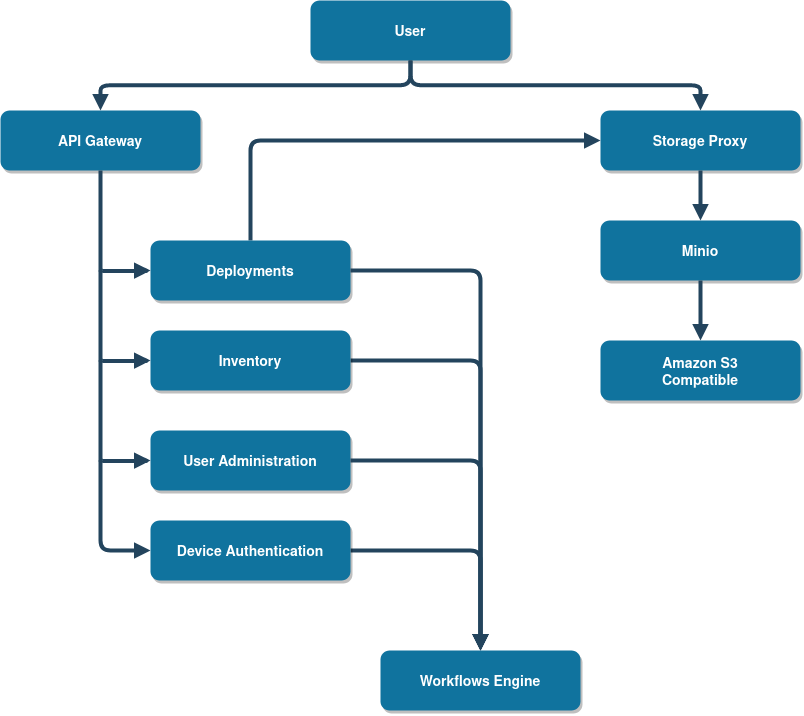
\includegraphics[scale=0.5]{images/integration-app.png}
    \caption{Mender Integration Server Architecture}
    \label{fig:mender-integration}
\end{figure}
Minio is a third-party object storage. It can either be used to serve uploaded content on its own or to proxy requests to Amazon S3 compatible cloud providers. All other services are mender application logic web services.
\newpage

\begin{figure}
    %\import{gen/}{example}
    \caption{Example Code Listing}
    \label{code:example-label}
\end{figure}

Listing \ref{code:example-label} is a very good YAML file.
